\documentclass[../piano-di-progetto.tex]{subfiles}

\begin{document}
\section{Modello di sviluppo}
Per lo sviluppo del progetto viene adottato il \textbf{modello incrementale} per garantire la qualità, conformità e maturità del prodotto.
\subsection{Il modello incrementale}
Nel modello di sviluppo incrementale, si suddivide lo sviluppo del sistema in \glossario{incrementi}, ognuno dei quali produce valore aggiunto. Le funzionalità corrispondenti ai requisiti fondamentali saranno sviluppate prima rispetto alle funzionalità opzionali. Dopo ogni incremento, si ottiene una versione del prodotto funzionante anche se, eventualmente, incompleto. L’aggiunta, modifica e cancellazione di requisiti sono possibili solamente dopo l'approvazione del proponente e mai durante lo sviluppo dell'incremento.

Questo modello presenta i seguenti vantaggi:
\begin{itemize}
    \item I requisiti vengono classificati in base alla loro importanza strategica affinché i più importanti abbiano precedenza sugli altri;
    \item Dopo ogni incremento è possibile ricevere un feedback da parte del proponente;
    \item L'attività di verifica è mirata alle modifiche dell'incremento attuale, ciò rende la verifica veloce ed economica;
    \item Ogni incremento riduce il rischio di fallimento mediante un approccio più realistico e predisposto ai cambiamenti.

\end{itemize}

\begin{figure}[H]
	\centering
    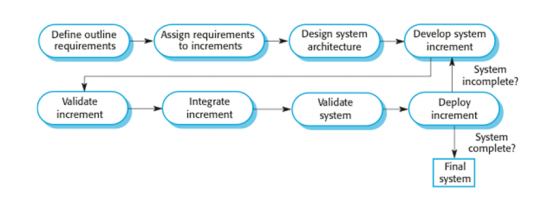
\includegraphics[width=16cm]{img/modello-incrementale.png}
    \caption{Diagramma del modello incrementale} 
	\label{fig:modello-incrementale}
  \end{figure}
  
  \subsection{Pianificazione di incremento}
  Ogni incremento verrà considerato come \emph{periodo} nel quale verranno svolte le attività riportate nei rispettivi diagrammi di Gantt. Ogni periodo viene strutturato come segue:
  \begin{itemize}
      \item \textbf{Riunione preliminare}: discussione e assegnazione delle attività da svolgere;
      \item \textbf{Svolgimento delle attività};
      \item \textbf{Verifica e revisione}: verifica di tutte le attività svolte nel periodo e valutazione dei risultati. 
  \end{itemize}

  \subsection{Incrementi}
  Di seguito vengono riportati gli incrementi programmati e i loro requisiti di riferimento. Ogni incremento verrà analizzato nella \S\ref{section:pian}.

  \begin{table}[H]
    \centering
    \begin{tabular}{cl}
        \rowcolor{lightgray}
    Incremento & Requisiti                                                                                                                                   \\
    I          &                                                                                                                                             \\
    II         & RFO1.4                                                                                                                                      \\
    III        & RFO1.1, RFO1.3, RFO1.3.2                                                                                                                    \\
    IV         & RFO1.1, RFO3.3,RFO3.3.1, RFO3.3.2, RFO7                                                                                                     \\
    V          & RFO1.3.1                                                                                                                                    \\
    VI         & RFO1.2, RFO1.5, RFO3, RFO3.1, RFO3.2                                                                                                        \\
    VII        & RFO4, RFO4.1, RFO4.2                                                                                                                        \\
    VIII       & \begin{tabular}[c]{@{}l@{}}RFD1.1.1, RFD1.2.1, RFD3.1.1, RFD3.1.2, RFD3.2.1\\ RFD3.2.2, RFD3.3.3, RFD6, RFD6.1, RFD6.2, RFD6.3\end{tabular} \\
    IX         & RFF1.3.2.1, RFF1.3.2.2, RFF5, RFF5.1, RFF5.2, RFF5.2.1, RFD5.2.1.1                                                                         
    \end{tabular}
    \caption{Tabella riassuntiva degli incrementi}
    \end{table}
\end{document}
